\section{Data Processing}
\label{sec:dataproc}

\subsection{Workflow}

The raw data from the detector subsystems is currently first preprocessed in what is called the decoding
stage. This is an I/O-heavy, single-threaded process and involves extracting hits from waveforms, translating
data-acquisition/hardware nomenclature (associated with crate/slot/channel labels) into physical detector objects,
performing special analyses dependent on serial event access, and converting from the input EVIO format to the
HIPO data format.  This phase includes registering beam helicity state changes and special scaler events, and
populating their results into special tagged HIPO events to facilitate later analysis.  The result is a factor of
$\sim$5 reduction in size and a file format optimized for I/O.

The second data processing stage is a CPU-heavy reconstruction phase, including all of the tracking, clustering,
calorimetry, time-of-flight, and event building described in the previous sections.  It runs multi-threaded in the
CLARA framework and can be configured to output various data schema depending on the purpose, see
Section~\ref{sec:dsts}, during full-scale data processing, or larger, special-purpose banks during preliminary
calibration phases.

The final stage of data processing involves the running of I/O-heavy analysis trains that perform event skimming
(e.g. filtering out specific final state event topologies),  and accommodate various corrections and common analysis
plugins.  It splits the data into multiple output files based on different event selections, each optimized for a
group of physics analyses. An example schematic is shown in Fig.~\ref{fig:train}. This stage is designed to be run
repeatedly as selection criteria and physics analyses mature. The reduction factor of the input file size generated
by the analysis trains depends directly on the applied filtering conditions for the specific output. Selecting events
with an electron identified in the ECAL provides a reduction factor of $\sim$0.3, while for events with an electron
in the ECAL and a positive hadron in CLAS12, the reduction factor is $\sim$0.1.  A typical 2~GB EVIO file gets
reduced to a 200~MB skimmed output HIPO data file.

\begin{figure}
    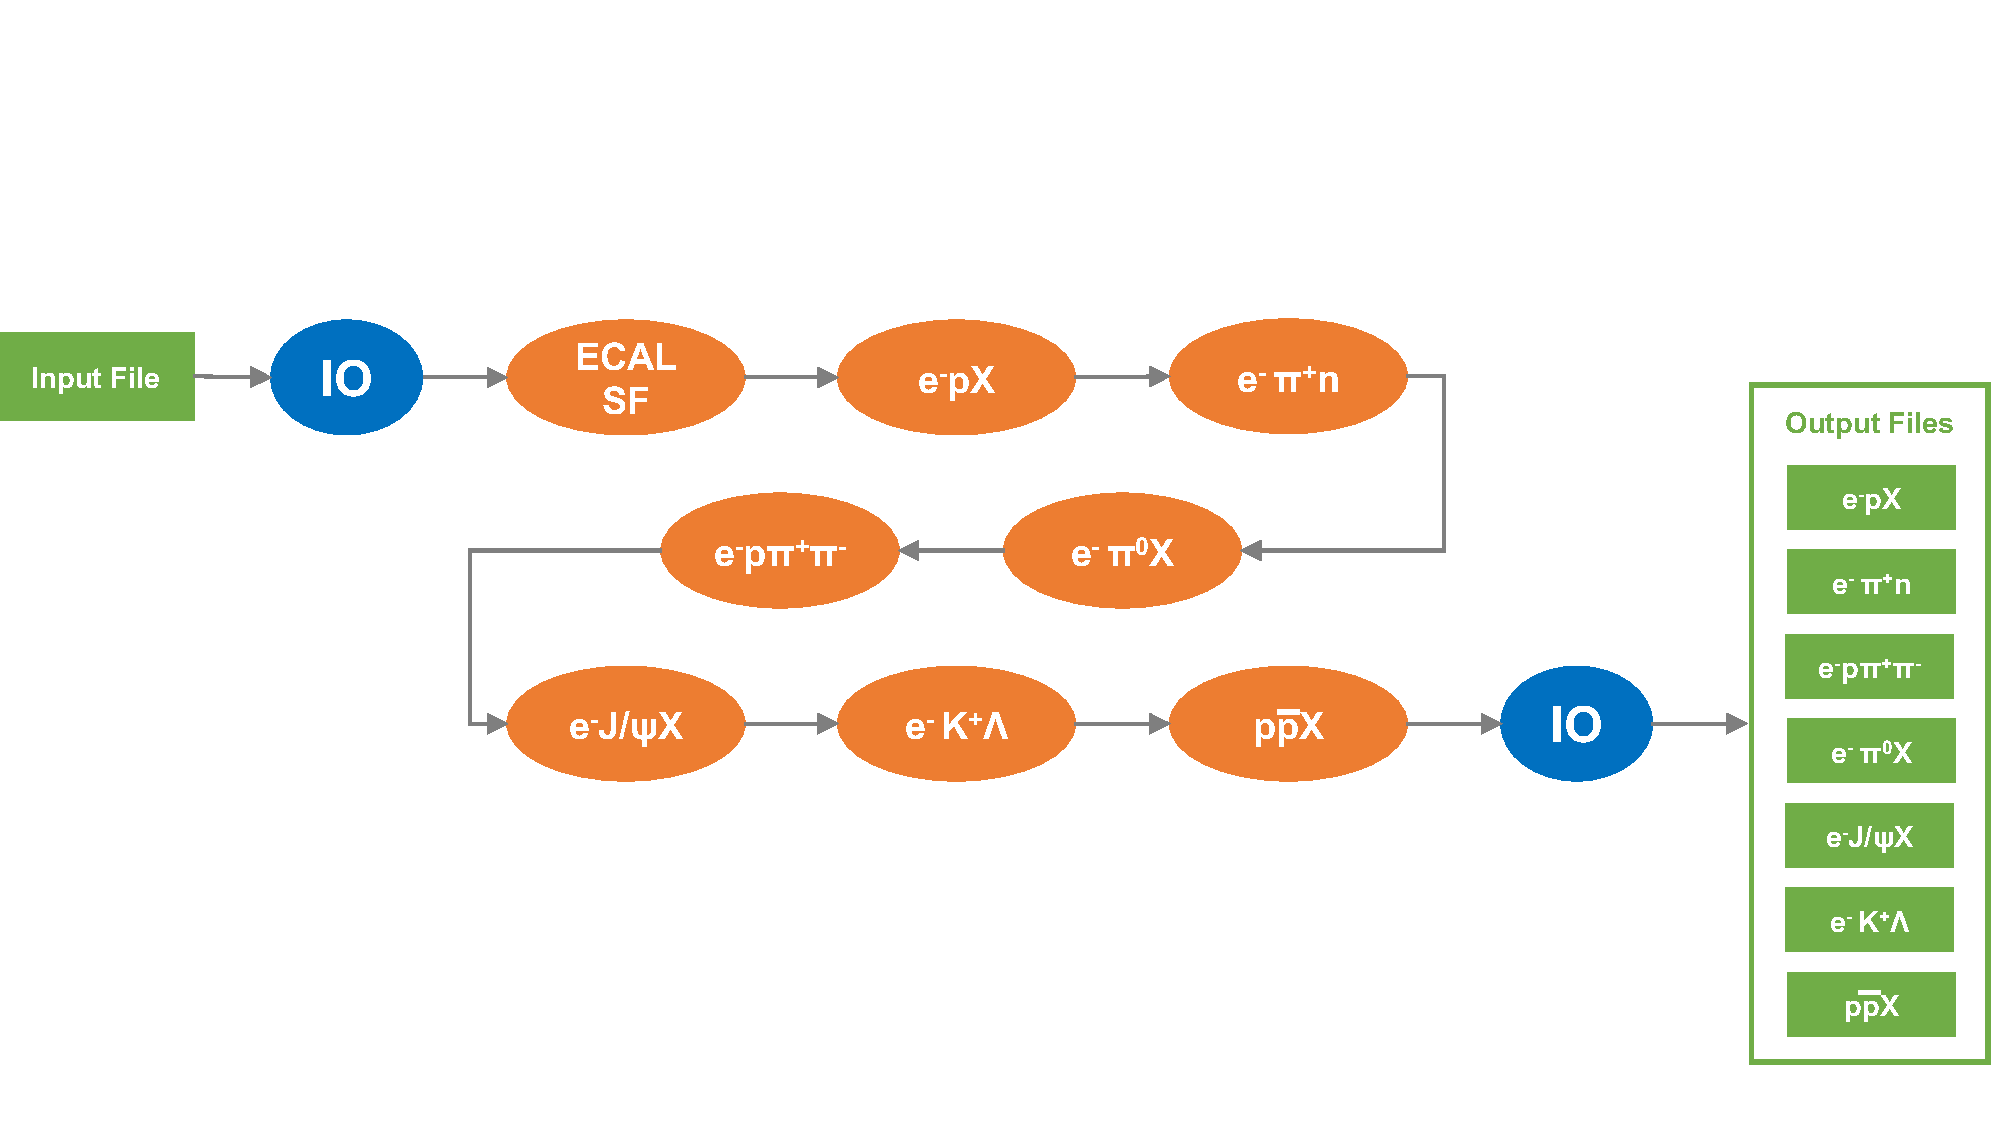
\includegraphics[width=0.45\textwidth,height=0.2\textheight]{pics/train.pdf}
    \caption{Schematic flow of analysis trains. The example shows a train composed of a plugin to correct the ECAL
      sampling fraction (SF) and several analysis filters for different final states. Events from a HIPO file are read
      by the IO service and processed through the analysis chain that applies the selected corrections and labels them
      according to the different filters. The labeled events are written to the corresponding output file.\label{fig:train}}
\end{figure}

\subsection{Data Summary Tapes}
\label{sec:dsts}

The final data output is provided by the Event Builder in the form of data summary tapes (DSTs), a standardized
selection of HIPO banks for physics analysis. The trains mentioned above are run on input DST files to produce
skimmed output DSTs. These include:

\begin{itemize}
\item global event information, e.g. run number and event time stamp, integrated beam charge, beam helicity state,
  event start time;
\item particle information, e.g. momentum four-vector and vertex position, particle type and identification quality,
  and status words that encode information on the sub-detectors involved in the particle formation;
\item high-level detector response information associated with each particle, e.g. detector identifier, response
  position and time, and track trajectory in each detector layer.
\end{itemize}

\noindent
The DST banks are organized such that the large detector information banks can easily be dropped to leave only
the data essential for a high-level physics analysis, without leaving unassociated references or unnecessary information.

\subsection{Computing Resources}

Reconstruction of all CLAS12 data is performed on Jefferson Lab's batch computing system~\cite{jlab-batch-farm}.
It currently consists of about 400 computing nodes of various types, with a total of about 21,000 available jobs
slots and half as many cores.  The input raw data and analyzed output data are stored on JLab's tape silo
\cite{jlab-tape-silo}, which provides sufficient cold storage for all of JLab's activities.  Data for physics analysis are
also stored live on JLab's Lustre filesystems~\cite{jlab-lustre}, which currently amounts about 2~PB of disk, but will
be increased to almost 7~PB in the near future. Analysis of the reconstructed data is performed on the JLab batch and
interactive farm nodes, and also exported to other institutions for final physics analysis. CLAS12 currently has 450~TB
available on different file systems, and a fair share computing resource of 36M~core-hr/yr.
